\capitulo{6}{Conclusiones}

En este proyecto, se han logrado alcanzar los objetivos planteados mediante un enfoque metódico y colaborativo. Los objetivos conseguidos son:
\begin{itemize}
    \item Comprender el funcionamiento del dispositivo Emotiv MN8 y para ello, se ha realizado una investigación profunda sobre el dispositivo y varias pruebas para entender completamente cómo funciona.
    \item Familiarizarse con los métodos de recopilación y análisis y para ello se han realizado varias pruebas con las aplicaciones de Contour y Emotiv, concretamente Emotiv Labs.
    \item Diseñar y realizar una serie de experimentos en el entorno de PsychoPy y para ello se ha tratado de emplear el PsychoPy Coder, pero se han experimentado muchos problemas y no se puede conseguir un resultado válido. Por lo tanto, se ha utilizado el PsychoPy Builder, permitiendo el diseño del experimento de una forma más sencilla.
    \item Evaluar la validez del dispositivo MN8 para su uso en el ámbito sanitario, el cual no se ha realizado específicamente pero hay estudios y artículos que indican la validez de los dispositivos Insight y EPOC X en este ámbito, lo que sugiere que los datos recopilados por el MN8 también son válidos.
    \item Contribuir a la comprensión de cómo se pueden utilizar los dispositivos EEG portables en la práctica sanitaria. Para ello, se ha realizado una investigación profunda sobre el dispositivo, aplicaciones y limitaciones entre otras cosas.
    \item Usar las herramientas de GitHub y Overleaf durante el desarrollo del proyecto, permitiendo un seguimiento y realización de toda la documentación del TFG.
    \item Analizar costes y viabilidad legal y para ello se ha realizado una investigación de todos los componentes necesarios así como las leyes que pueden afectar al proyecto.
    \item Realizar un trabajo reproducible en el futuro. Para hacer esto posible, se ha realizado la documentación de la forma más clara y explicativa posible, tanto de Emotiv como de PsychoPy.
\end{itemize}

\section{Aspectos relevantes.}

Este apartado pretende recoger los aspectos más interesantes del desarrollo del proyecto, incluyendo los detalles más relevantes en cada fase del desarrollo, justificando los caminos tomados, especialmente aquellos que no sean triviales. Hay que tener en cuenta que estos problemas o modificaciones producidas pueden haber sido causados por las características de los materiales antialérgenos o su tratamiento, ya que en otros dispositivos, como los del laboratorio, no ha sido necesario.

\subsection{Problemas de conexión intermitente con Emotiv Insight.}
\subsubsection{Descripción del problema.}
Durante la semana del Objetivo 5, mientras realizaba el proceso de conexión del Emotiv Insight con el ordenador, he experimentado un problema técnico. Aunque inicialmente se puede establecer una conexión exitosa y observar los EEG en tiempo real, la conexión se perdió después de aproximadamente un minuto. Este patrón se repitió a pesar realizar varios intentos de reconexión, así como reinicio del ordenador, lo que imposibilitó la realización de grabaciones e investigaciones necesarias.

\subsubsection{Detalles del error.}
El dispositivo Insight se conecta correctamente al ordenador y permite la visualización de los EEG en tiempo real. Sin embargo, tras aproximadamente un minuto, se pierde la conexión entre ambos. A pesar de los intentos de reconexión, este problema persiste y dificulta la realización del proyecto.

\subsubsection{Posibles causas del error.}
Las posibles causas del error podrían ser:
\begin{itemize}
    \item En ciertas ocasiones, si el Insight no establece una conexión Bluetooth que permita tanto la voz como la música, puede ocurrir que no se pueda reconectar durante la misma sesión. Además, se han observado casos en los que el dispositivo ha logrado conectar la BCI pero no la función de música. Sin embargo, esta última situación parece haber ocurrido antes de las últimas actualizaciones del \textit{software}.
    \item Otra posibilidad es que el \textit{software} del Insight se pueda vincular y utilizar únicamente en un ordenador, limitando su uso exclusivamente en ese dispositivo.
\end{itemize}

\subsubsection{Acciones tomadas.}
Lo primero que se ha intentado para superar el error de desconexión que se experimentado con el Emotiv Insight, es realizar pruebas utilizando un dispositivo de Bluetooth 5.0 conectado a mi ordenador personal. Este paso tiene como objetivo determinar si el uso de una versión más avanzada de Bluetooth puede mejorar la conectividad del dispositivo.

A pesar de utilizar el dispositivo de Bluetooth 5.0, el problema persiste. Por lo tanto se ha probado a realizar la conexión del dispositivo con el ordenador del laboratorio, con y sin el dispositivo Bluetooth 5.0, y no ha sido posible realizarla de forma exitosa, concluyendo que queda descartada la posibilidad de que el problema provenga de la conexión.

Después de las pruebas en el laboratorio, se concluye que el dispositivo no es reconocido en los distintos sistemas, por lo que se probará en el dispositivo en el que se realizaron las primeras pruebas.

Tras los errores presentados y a pesar de los intentos de reiniciar el \textit{software}, el dispositivo se entrega al tutor del TFG (Pedro Luis Sánchez Ortega) y tras realizar diversas pruebas, obtiene un aviso de límite de dispositivos alcanzado, como se puede observar en la imagen \ref{fig: LimiteDispositivos}.

\begin{figure}[H]
    \centering
    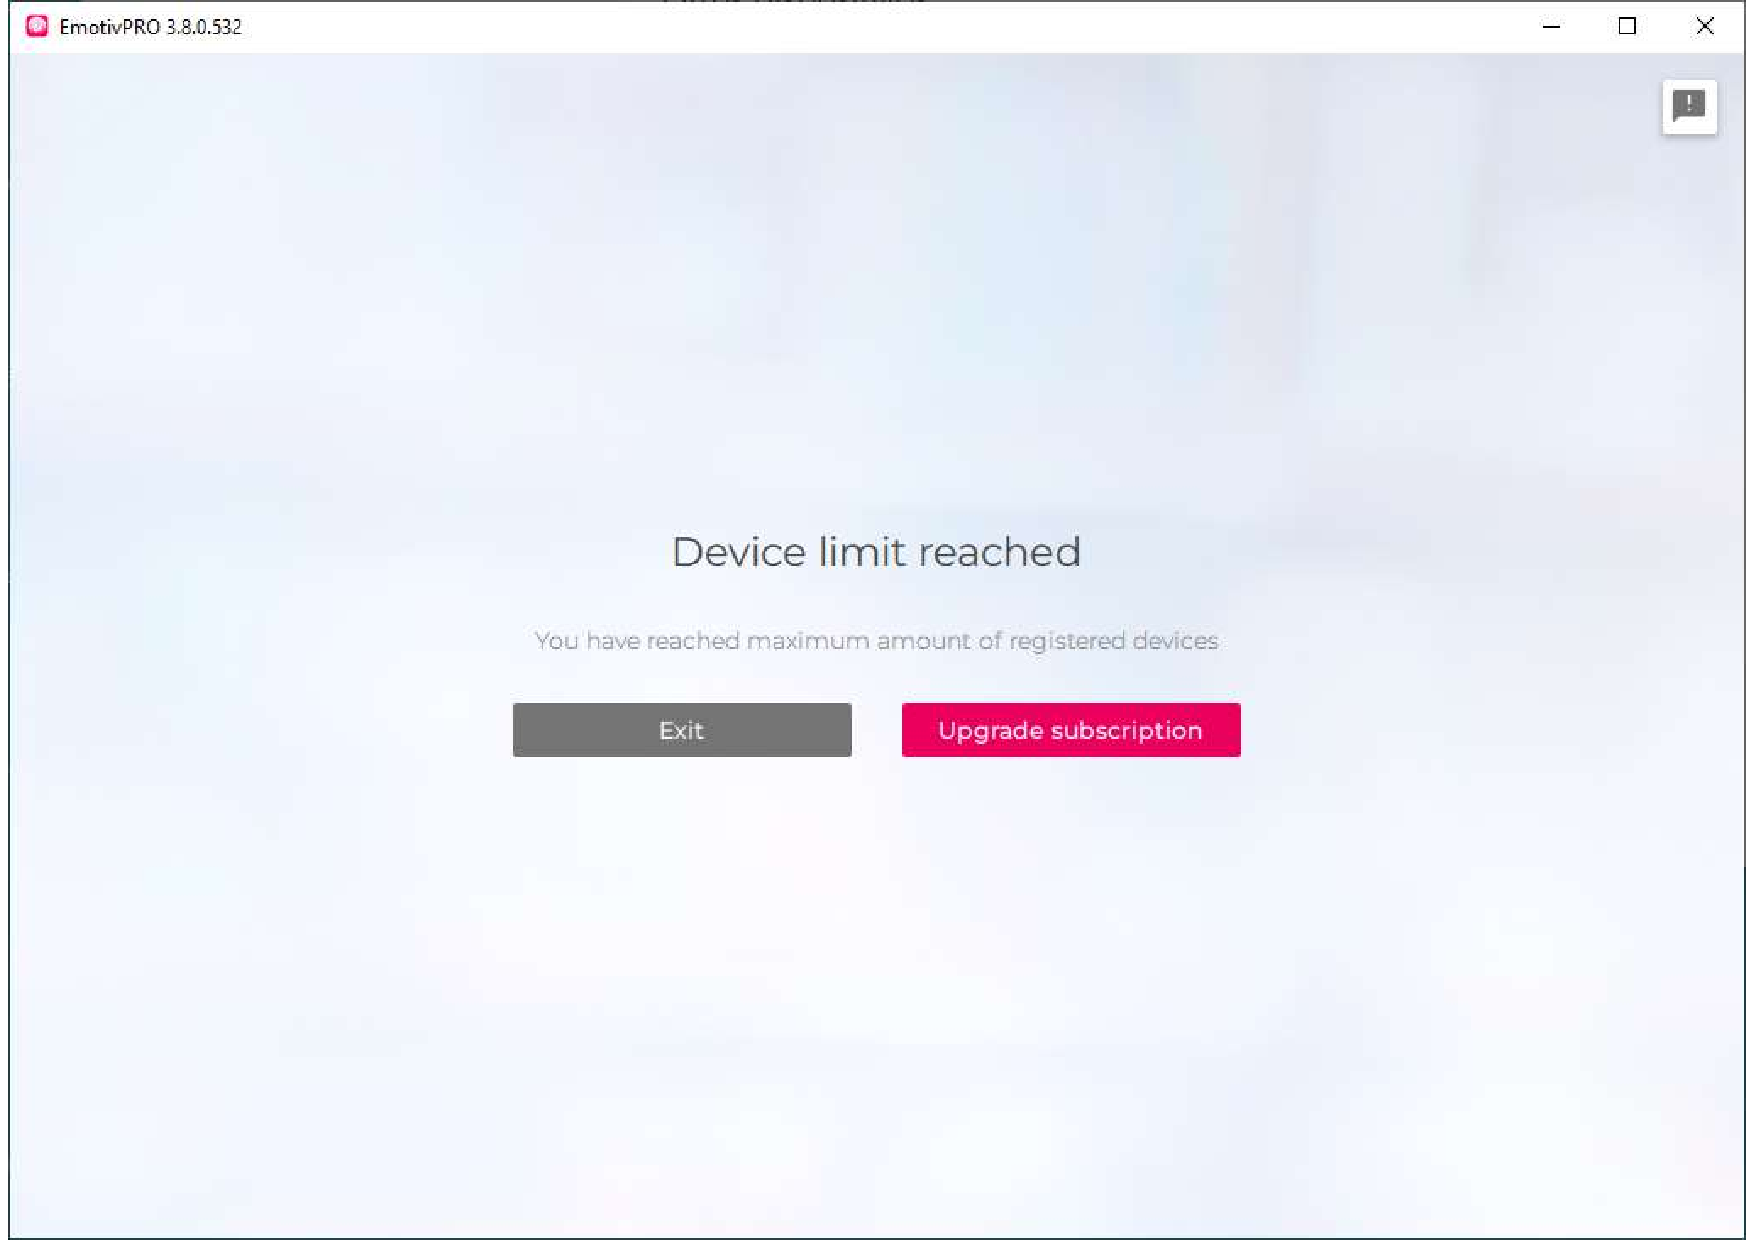
\includegraphics[width=0.4\textwidth]{img/LimiteDispositivosEmotiv.pdf}
    \caption{Aviso de límite de dispositivos alcanzado.}
    \label{fig: LimiteDispositivos}
\end{figure}

Por lo tanto, tras la acumulación de varias horas de pruebas e investigación, se comprueba la hipótesis de que la licencia y la primera conexión limitan el uso del dispositivo a un solo ordenador. Otra conclusión que se puede sacar de ello es que su uso para terapia queda limitado, ya que el dispositivo está destinado a ser empleado en un único ordenador con un único usuario que posea las licencias adecuadas; cabiendo la posibilidad de mejorar las licencias, lo que implica pagar más dinero.

\subsection{Problema conexión MN8.}
Durante el proceso de conexión del dispositivo MN8 con el ordenador, se experimentó un problema técnico. El dispositivo MN8 se conectaba correctamente al ordenador, pero dentro de la configuración y posicionamiento del dispositivo, la calidad de la señal era del 0\%. Esto implicaba que, a pesar de que el dispositivo era detectado, no había una comunicación efectiva entre el dispositivo y el ordenador.

Para resolver este problema, se realizó un cambio de sensores por los que tienen 3 filamentos, lo que aumentó la superficie de contacto. Este cambio permitió finalmente una calidad de conexión óptima del 100\%.

Tras el cambio de sensores, se obtuvo una correcta solución al problema. La calidad de la conexión entre el dispositivo MN8 y el ordenador mejoró significativamente, pasando de un 0\% a un 100\%. Esto permitió una comunicación efectiva entre el dispositivo y el ordenador, facilitando así la realización de las tareas necesarias. Por lo tanto, se concluye que el cambio de sensores fue una solución efectiva para el problema experimentado.

\subsection{Problema con PsychoPy Coder.}
El experimento fue inicialmente diseñado con PsychoPy Coder, que es un entorno de programación con código para la realización de experimentos que permite el uso de dispositivos de Emotiv para la lectura de EEG. En este entorno se generaba un error en la conexión con el dispositivo Emotiv que no permitía ni la lectura de EEG ni la correcta ejecución del experimento. A partir de este problema se decidieron probar las mismas rutinas diseñadas en PsychoPy Builder, que es el entorno de programación por bloques de PsychoPy. De esta manera no se obtienen errores en la ejecución y pueden visualizarse sin problema todas las rutinas del experimento y añadir el componente de\textit{ Emotiv Recording}.
